\section{Power consumption esitmation}
In this section, there is a description of the power consumption of the ESP32 node in all states: deep sleep, idle, sensor reading, WiFi turned on and transmission.\\
In order to estimate power consumption based on the provided CSV files, we first plotted data using Python and Matplotlib library. Based on the plot, we computed the average power consumption in the analyzed working state.

\subsection{Power consumption data plots}
In order to plot the data contained in the provided CSV files, we used the following algorithm.

\begin{python}
import pandas as pd
import matplotlib.pyplot as plt
# read CSV file 
df = pd.read_csv('deep_sleep.csv', parse_dates=['Timestamp'])
# plot data
plt.figure(figsize=(10, 6))
plt.plot(df['Timestamp'], df['Data'], linestyle='-', linewidth=2)
plt.xlabel('Time')
plt.ylabel('Power [mW]')
plt.title('Power consumption deep sleep')
plt.grid(True)
# save and shows
plt.savefig("power_consumption_deep_sleep.pdf", format="pdf", bbox_inches="tight")
plt.show()
\end{python}

\subsubsection{Power consumption deep\_sleep.csv}
The following plot represents the power consumption when the ESP32 is in deep sleep state (lowest power level), goes into idle mode (medium power level) and finally turns the WiFi on (highest power level). 
\begin{figure}[H]
    \centering
    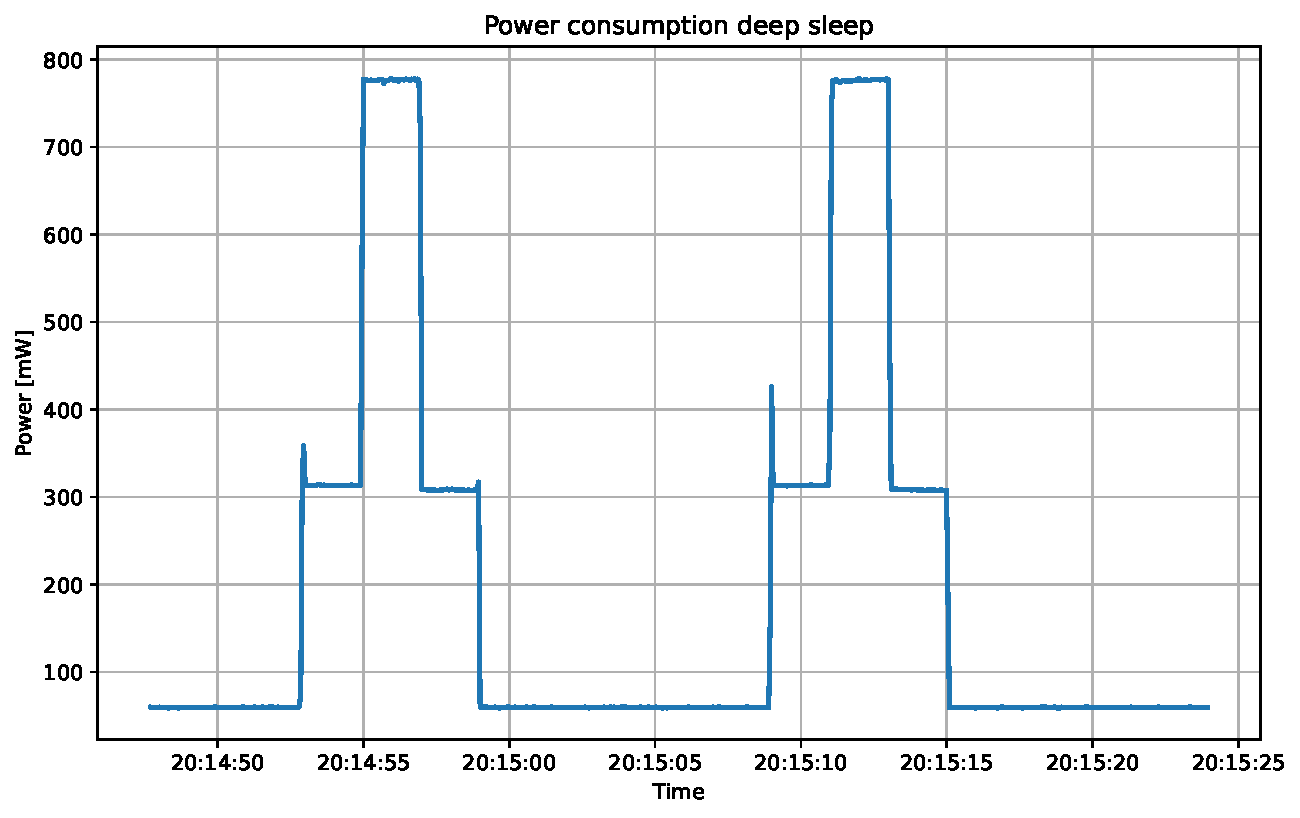
\includegraphics[width=\linewidth, height=0.4\textheight, keepaspectratio]{power_consumption_deep_sleep.pdf}
    \caption{Power consumption deep sleep state}
    \label{fig:Power consumption deep sleep state}
\end{figure}

\subsubsection{Power consumption sensor\_read.csv}
The following plot represents the power consumption when the ESP32 alternates the idle mode and sensor reading mode, in which it performs a measurement using the Ultrasonic Distance Sensor HC-SR04.
\begin{figure}[H]
    \centering
    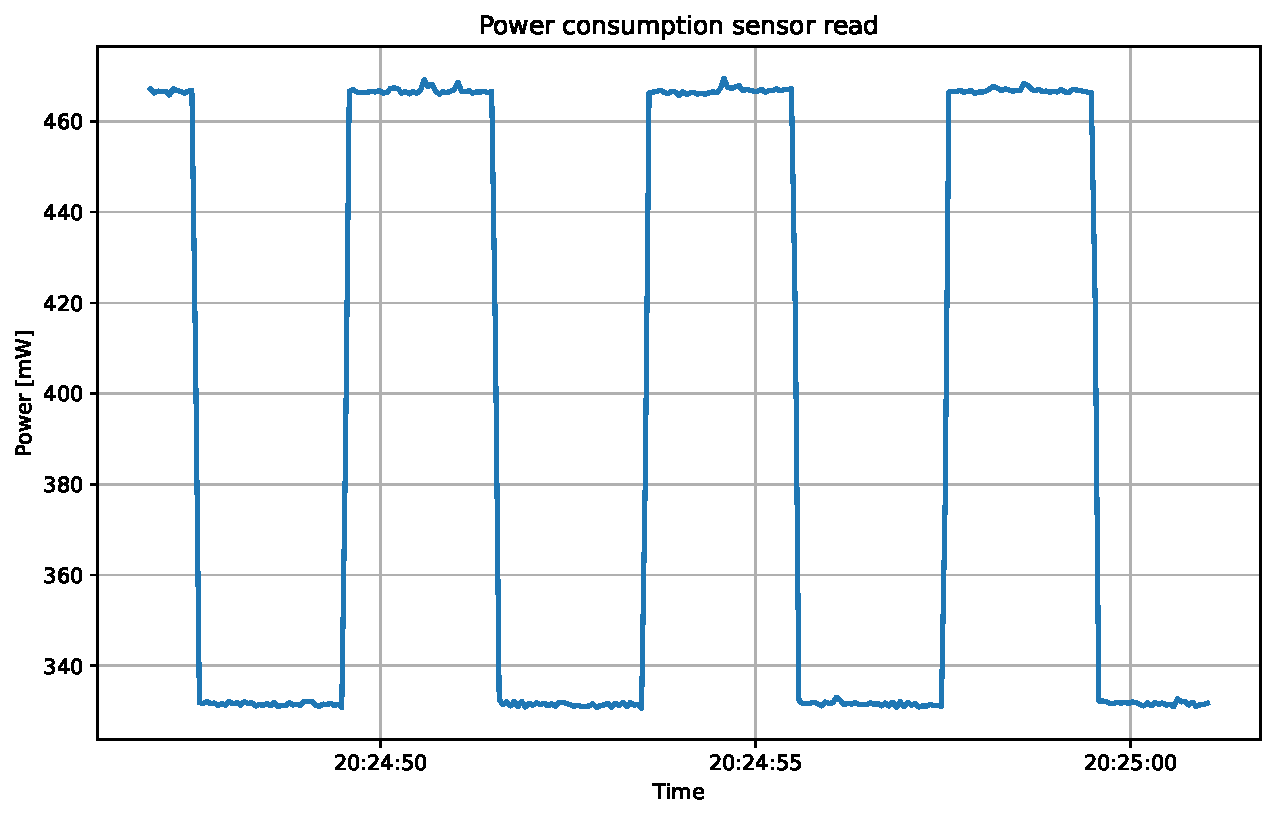
\includegraphics[width=\linewidth, height=0.4\textheight, keepaspectratio]{power_consumption_sensor_read.pdf}
    \caption{Power consumption deep sleep state}
    \label{fig:Power consumption deep sleep state}
\end{figure}

\subsubsection{Power consumption transmission\_power.csv}
The following plot represents the power consumption when the ESP32 has the WiFi turned on and transmits data using ESP-NOW at 19.5 dBm and 2 dBm.
\begin{figure}[H]
    \centering
    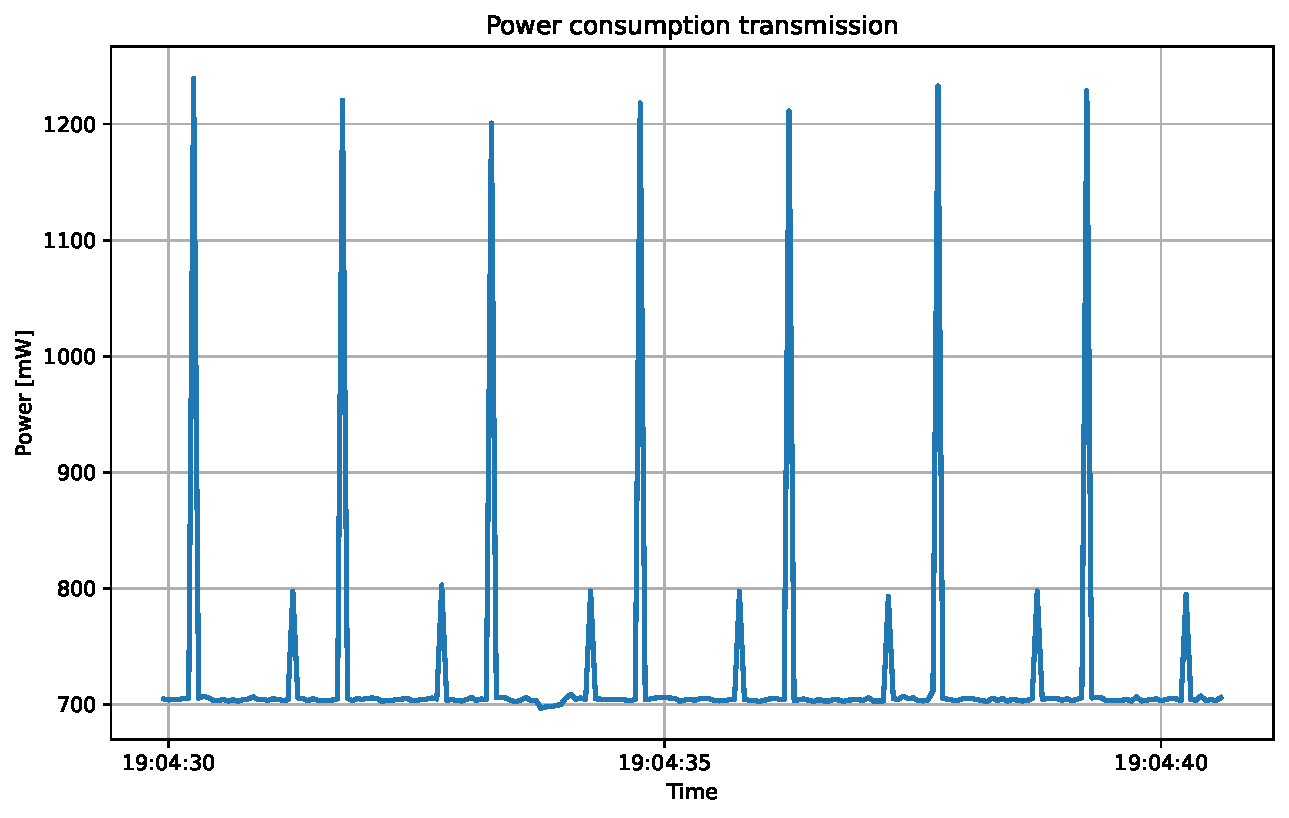
\includegraphics[width=\linewidth, height=0.4\textheight, keepaspectratio]{power_consumption_transmission.pdf}
    \caption{Power consumption deep sleep state}
    \label{fig:Power consumption deep sleep state}
\end{figure}

\subsection{Numerical power consumption estimation}
In order to find a numerical estimation of the power consumption in different states, we used some Python algorithms, using the library Pandas. Starting from the plot we selected the range of values regarding a particular state, discarding the others, and computed the average power consumption. For some states, the values of power can be found in multiple CSV files; in such cases, we merged different files in order to have a more accurate estimation.\\
In the following sections we also report two example of algorithms used to compute the average, both using a single dataset and multiple datasets.

\subsubsection{Power consumption in deep sleep state}
Data to estimate the deep sleep mode is contained in the dataset deep\_sleep.csv. We filtered all values of power above 100mW, referring to other states as shown by the plot, and computed the average.

\begin{python}
import pandas as pd 
# read CSV file 
dataset_deep_sleep = pd.read_csv("deep_sleep.csv", parse_dates=['Timestamp'])
# filter data with power < 100mW, referring to deep sleep mode
deep_sleep_data = dataset_deep_sleep[dataset_deep_sleep["Data"] < 100]
# compute average
deep_sleep_avg_power = deep_sleep_data["Data"].mean()
# print average 
print("Average power consumption deep sleep: ", deep_sleep_avg_power)
\end{python}

We obtained an average consumption in deep sleep of 59.66 mW.

\subsubsection{Power consumption in idle state}
The power consumption in idle state can be extracted both by sensor\_read.csv and transmission\_power.csv. We used both datasets, merging all values and computing the average. We considered only values between 200 mW and 500 mW, that refer to idle mode.
\begin{python}
import pandas as pd 
# read CSV file 
dataset_deep_sleep = pd.read_csv("deep_sleep.csv", parse_dates=['Timestamp'])
dataset_sensor_reading = pd.read_csv("sensor_read.csv", parse_dates=['Timestamp'])
# filter data with power between 200mW and 500mW, referring to idle mode
idle_data_deep_sleep = dataset_deep_sleep[(dataset_deep_sleep['Data'] >= 200) & (dataset_deep_sleep['Data'] <= 500)]
# filter data with power <= 400mW, reffering to idle mode
idle_data_sensor_reading = dataset_sensor_reading[dataset_sensor_reading['Data'] <= 400]
# merge values 
idle_merged = pd.concat([idle_data_deep_sleep, idle_data_sensor_reading], ignore_index=True)
# compute average
idle_avg_power = idle_merged['Data'].mean()
# print average 
print("Average power consumption idle: ", idle_avg_power)
\end{python}

We obtained an average consumption in idle of 322.62 mW.

\subsubsection{Power consumption in measurement state}
Data representing power consumption in measurement state is contained in the dataset sensor\_read.csv. We computed the average value considering values of power above 400 mW and obtained an average value of 465.18 mW. The algorithm is very similar to deep sleep mode, thus we don't report it.

\subsubsection{Power consumption in WiFi on state}
We estimated the power consumption when the WiFi is turned on and the ESP32 is not transmitting based on deep\_sleep.csv and transmission\_power.csv, merging all value between 600 mW and 750 mW, as shown for the idle mode. The average power consumption when WiFi is turned on is 724.58 mW.

\subsubsection{Power consumption when transmitting at 2 dBm}
Finally, we estimated the average power consumption when ESP32 is transmitting at 2 dBm, based on transmission\_power.csv. We compute the average of values between 750 mW and 900 mW, obtaining an average value of 797.29 mW.


Power consumption estimation
Deep sleep duration: 48 s
Average Idle duration: 833.6985294117648 uS
Average Measurement duration: 18647.79411764706 uS
Average WiFi duration: 188640.86842105264 uS
Average Sending duration: 59.6044776119403 uS

Battery size
18593 J

Average power consumption 
Average power consumption deep sleep:  59.66093555093555 mW
Average power consumption idle:  322.62464743589743 mW
Average power consumption measurement:  465.18097744360904 mW
Average power consumption WiFi on:  724.5793571428571 mW
Average power consumption transmission at 2dBm:  797.2942857142858 mW
